\subsection{Scalability}
\label{sec:exp-scalability}

Finally, we confirm that NESS is practical at scale. Figure~\ref{fig:scalability} plots test macro-F1 against peak GPU memory for all methods on ogbn-arxiv, with bubble size indicating training time. NESS attains the highest accuracy at a peak memory of $1.3$~GB, comparable to the per-node baseline (MATE) and well within a single GPU; its self-supervised objectives and prefill add no memory penalty relative to a standard clustered GNN. Its training time is higher than the simpler baselines (larger bubble), reflecting the auxiliary objectives computed each epoch, but remains on the order of minutes on a single GPU.

\begin{figure}[t]
\centering
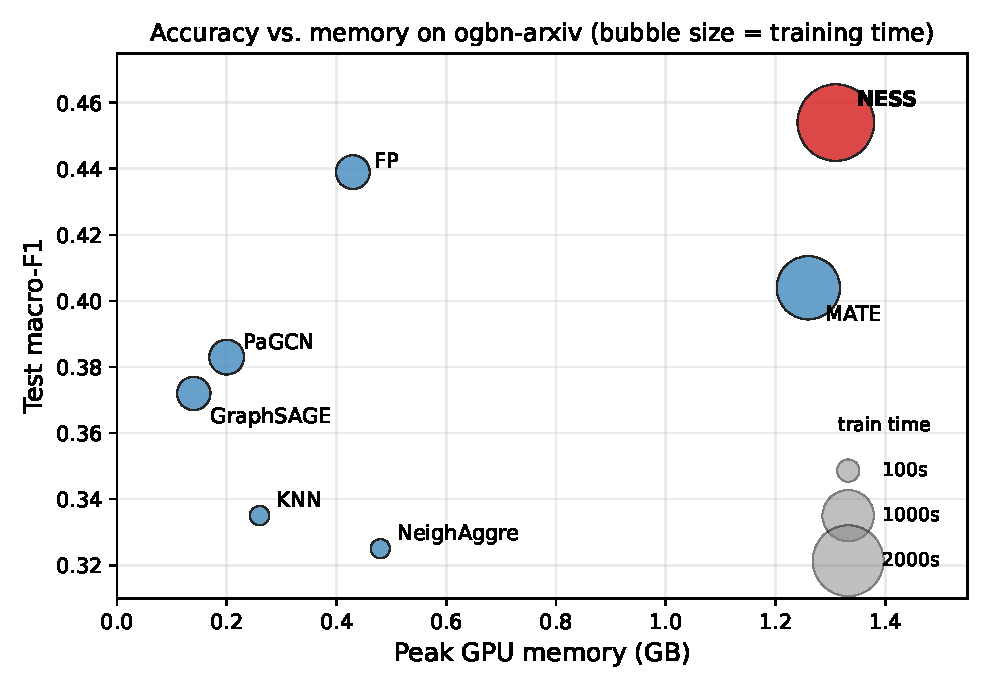
\includegraphics[width=0.95\linewidth]{figures/e6_scalability_bubble.pdf}
\caption{Accuracy versus peak GPU memory on ogbn-arxiv; bubble size is training time. NESS (red) attains the highest macro-F1 at memory comparable to other GNNs, confirming it scales without a memory penalty. Memory and time are measured at $80\%$ missingness; accuracy is the main-comparison result (Table~\ref{tab:main}).}
\label{fig:scalability}
\end{figure}
